\documentclass[aspectratio=1610]{beamer}
\usetheme{Madrid}
\usepackage{xeCJK}
\setCJKmainfont{SimSun}
\usepackage{multirow}
\usepackage{graphicx}
\usepackage{booktabs} % for better table formatting
\usepackage{geometry} % for adjusting page layout
\usepackage{enumitem} % for customizing lists
\usepackage{hyperref} % for clickable links and references
\usepackage{subcaption}

\title[program test]{硕士中期报告-软件测试}
\author[Gcc]{高丁超}
\institute[ISCAS]{Institute of Software Chinese Academy of Sciences}

\begin{document}
\begin{frame}[plain]
  \titlepage
  %  Title page
\end{frame}
\begin{frame}{背景介绍}
    \begin{itemize}
        \Large
        \item  transition system: $(S, I, \Sigma, T)$
        \begin{equation}
          where
          \begin{cases}
            x = x_1, \cdots, x_n\\
            y = y_1, \cdots, y_n\\
            \sigma = \sigma_1, \cdots, \sigma_m
          \end{cases}
          \notag
        \end{equation}
        \item Quantum transition system: $(S, S_0, \Sigma, R)$
    \end{itemize}
\end{frame}

\begin{frame}{前期调研}
    \begin{figure}
        \centering
        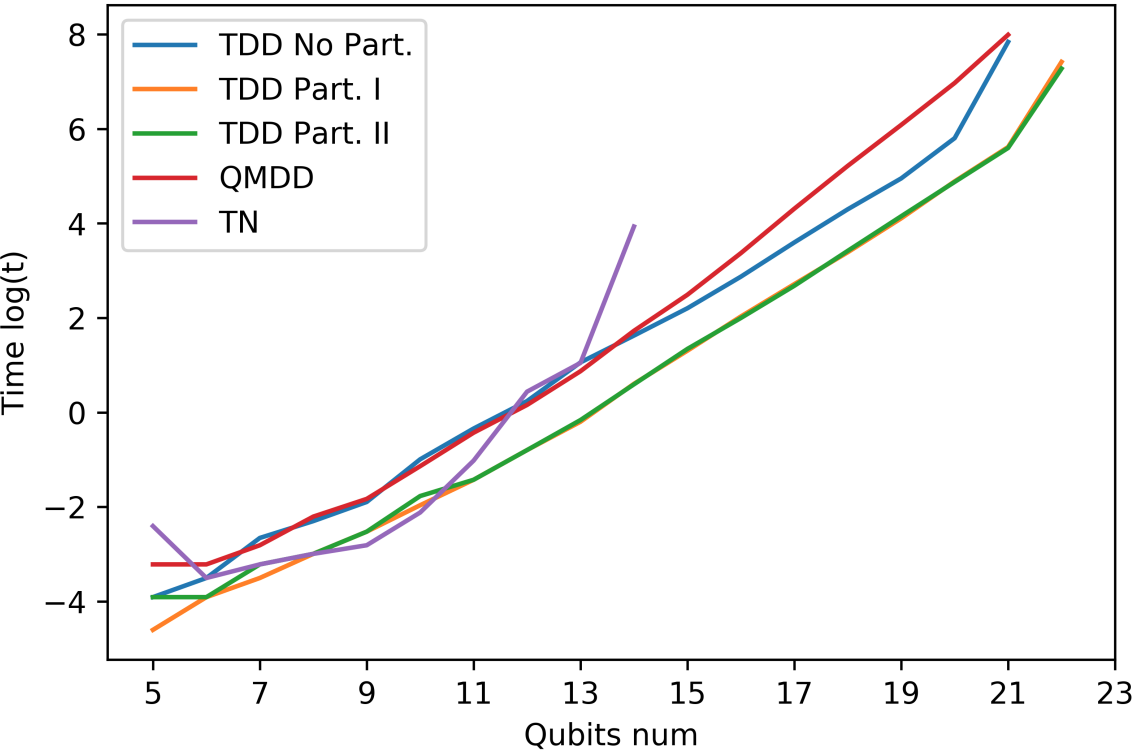
\includegraphics[width=.8\textwidth]{Img/tdd-compare.pdf}
    \end{figure}
\end{frame}
\begin{frame}{基本功能}
    \begin{figure}
        \centering
        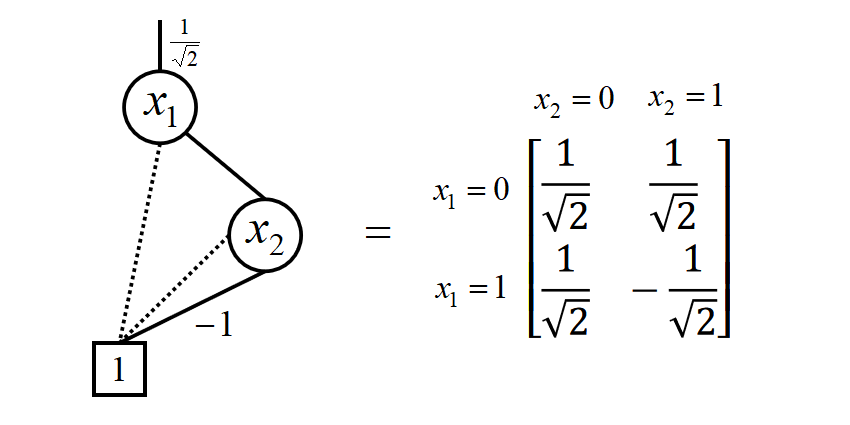
\includegraphics[width=.8\textwidth]{Img/TDD_H_gate2.png}
    \end{figure}
\end{frame}
\begin{frame}{模块功能}
    \begin{center}
        \begin{itemize}
            \item \textbf{输入处理模块}
            \item \textbf{内存管理模块}
            \item \textbf{TDD基础模块}
            \item \textbf{TDD算法模块}
        \end{itemize}
    \end{center}
\end{frame}
\begin{frame}{测试样例}
    \begin{table}[]
        \Large
        \rule{0pt}{30pt}
        \begin{tabular}{l|ccc}
        benchmark & basic & addition& contraction \\\hline
        Grover 20       & $\sim$5min  & $\sim$4min & $\sim$4sec  \\
        Quantum Fourier Transform 20           & $\sim$20min & $\sim$11min & $<$1sec \\
        Quantum Random walk 20           & $\sim$6min & $\sim$4min & $\sim$15sec\\
        Bernstein-Vazirani 50           & $\sim$4min & $\sim$4min & $\sim$16sec \\
        GHZ 500         & $\sim$3sec & $\sim$1.5sec & $\sim$1.7sec\\
        \end{tabular}
    \end{table}
\end{frame}
\begin{frame}{测试样例}
    \begin{figure}
        \centering
        \begin{subfigure}{0.4\textwidth}
            \centering
            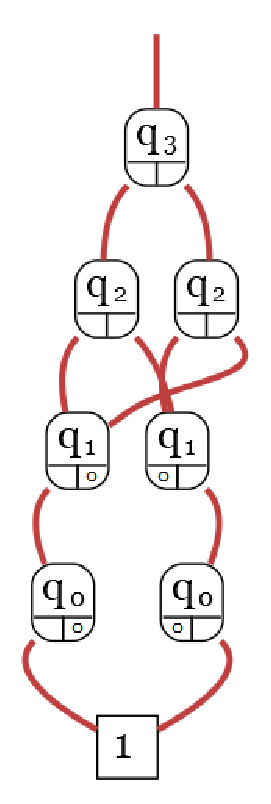
\includegraphics[height=8cm]{Img/cx.eps}
        \end{subfigure}
        \begin{subfigure}{0.4\textwidth}
            \centering
            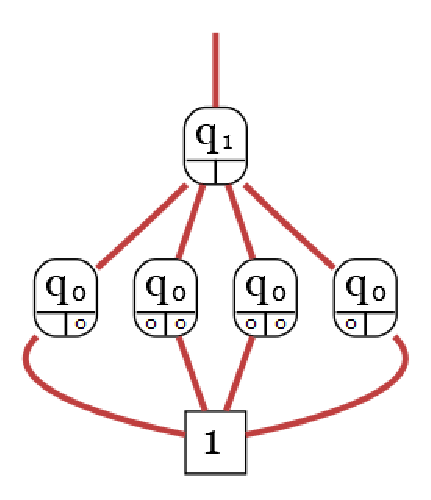
\includegraphics[height=8cm]{Img/cnot.eps}
        \end{subfigure}
    \end{figure}
\end{frame}
\end{document}